\documentclass{article}
\usepackage[margin=1in]{geometry}
\usepackage{amsmath}
\usepackage{amssymb}
\usepackage{amsthm}
\usepackage{bm}
\usepackage{hyperref}
\usepackage{graphicx}
\usepackage{caption}
\usepackage{listings}
\usepackage{xcolor}
\usepackage{float}
\usepackage{placeins}
\graphicspath{{figures/}}

% Code style
\lstdefinestyle{code}{
  basicstyle=\ttfamily\small,
  numbers=left,
  numberstyle=\tiny,
  numbersep=8pt,
  keywordstyle=\color{blue},
  commentstyle=\color{teal!70!black},
  stringstyle=\color{orange!70!black},
  showstringspaces=false,
  breaklines=true,
  frame=single,
  framerule=0.3pt,
  rulecolor=\color{black!15}
}
\lstset{style=code}

\title{Multimodal Foundation Models and Efficient Adaptation Techniques}
\author{}
\date{\today}

\begin{document}
\maketitle
\tableofcontents
\FloatBarrier

\section{CLIP, Flamingo, GPT-4, LLaVA}
Multimodal foundation models align vision and language representations at scale, enabling zero-shot recognition, image-conditioned generation, and interactive reasoning. Figure~\ref{fig:clip_multimodal_alignment} compares embedding spaces learned by representative architectures.

\subsection{Contrastive Language-Image Pretraining (CLIP)}
CLIP pairs an image encoder $f_{\theta}$ and text encoder $g_{\phi}$ trained on 400M image-text pairs. Given batch size $B$, embeddings $\mathbf{v}_i = f_{\theta}(\mathbf{x}_i)$ and $\mathbf{t}_i = g_{\phi}(\mathbf{y}_i)$ are normalized and optimized via symmetric cross-entropy:
\begin{align}
  \ell_{\text{img}} &= -\frac{1}{B} \sum_{i=1}^{B} \log \frac{\exp(\mathbf{v}_i^\top \mathbf{t}_i / \tau)}{\sum_{j=1}^{B} \exp(\mathbf{v}_i^\top \mathbf{t}_j / \tau)}, \\
  \ell_{\text{text}} &= -\frac{1}{B} \sum_{i=1}^{B} \log \frac{\exp(\mathbf{t}_i^\top \mathbf{v}_i / \tau)}{\sum_{j=1}^{B} \exp(\mathbf{t}_i^\top \mathbf{v}_j / \tau)}, \\
  \mathcal{L}_{\text{CLIP}} &= \frac{1}{2} (\ell_{\text{img}} + \ell_{\text{text}}).
\end{align}
Temperature $\tau$ is learned, improving sharpness of similarity scores. Zero-shot classification replaces linear classifiers with text prompts, $\hat{y} = \arg\max_{k} \mathbf{v}_\mathrm{test}^\top \mathbf{t}_k$, where $\mathbf{t}_k$ encodes ``a photo of a \{label\}''.

\subsection{Flamingo: Perceiver-based Vision-Language Model}
Flamingo combines a frozen vision encoder and language model via gated cross-attention layers (Gated XAttn-Dense). Given token sequence $\mathbf{h}_{\mathrm{LM}}$ and visual features $\mathbf{h}_{\mathrm{vis}}$, a layer computes
\begin{align}
  \mathbf{z} &= \mathrm{MultiHeadQK}(\mathbf{h}_{\mathrm{LM}}, \mathbf{h}_{\mathrm{vis}}), \\
  \mathbf{m} &= \sigma(\mathbf{W}_g [\mathbf{h}_{\mathrm{LM}}, \mathbf{z}]) \odot \mathbf{W}_m \mathbf{z}, \\
  \mathbf{h}'_{\mathrm{LM}} &= \mathbf{h}_{\mathrm{LM}} + \mathbf{m},
\end{align}
where $\sigma$ is sigmoid gating. The Perceiver Resampler distills variable-length visual tokens into a fixed set of latent vectors, enabling few-shot multimodal learning with minimal task-specific tuning.

\subsection{GPT-4 and Multimodal Extensions}
GPT-4 integrates visual understanding by fusing image embeddings through multimodal adapters. While architectural details remain proprietary, public descriptions emphasize:
\begin{itemize}
  \item Vision encoder producing patch tokens passed to a projection layer aligning with transformer embeddings.
  \item Joint positional encodings allowing interleaved text and visual tokens.
  \item Reinforcement learning from human feedback (RLHF) on multimodal conversations.
\end{itemize}
The model excels at reasoning over charts, diagrams, and complex instructions, marking the shift toward generalist assistants.

\subsection{LLaVA: Large Language and Vision Assistant}
LLaVA fine-tunes a frozen CLIP vision encoder and Vicuna language model with visual instruction data. A projection matrix $W_{\text{proj}}$ maps pooled visual features $\mathbf{v}$ to language hidden size $d$:
\begin{equation}
  \tilde{\mathbf{v}} = W_{\text{proj}} \mathbf{v}, \quad \mathbf{H}_0 = [\text{BOS}, \tilde{\mathbf{v}}, \text{Text tokens}].
\end{equation}
Training uses a two-stage approach:
\begin{enumerate}
  \item \textbf{Visual instruction tuning:} SFT on GPT-generated dialogues describing images.
  \item \textbf{Alignment refinement:} Preference optimization (e.g., DPO) to align responses with human preferences.
\end{enumerate}
The model demonstrates strong performance on benchmarks such as ScienceQA and VizWiz.

\begin{figure}[H]
  \centering
  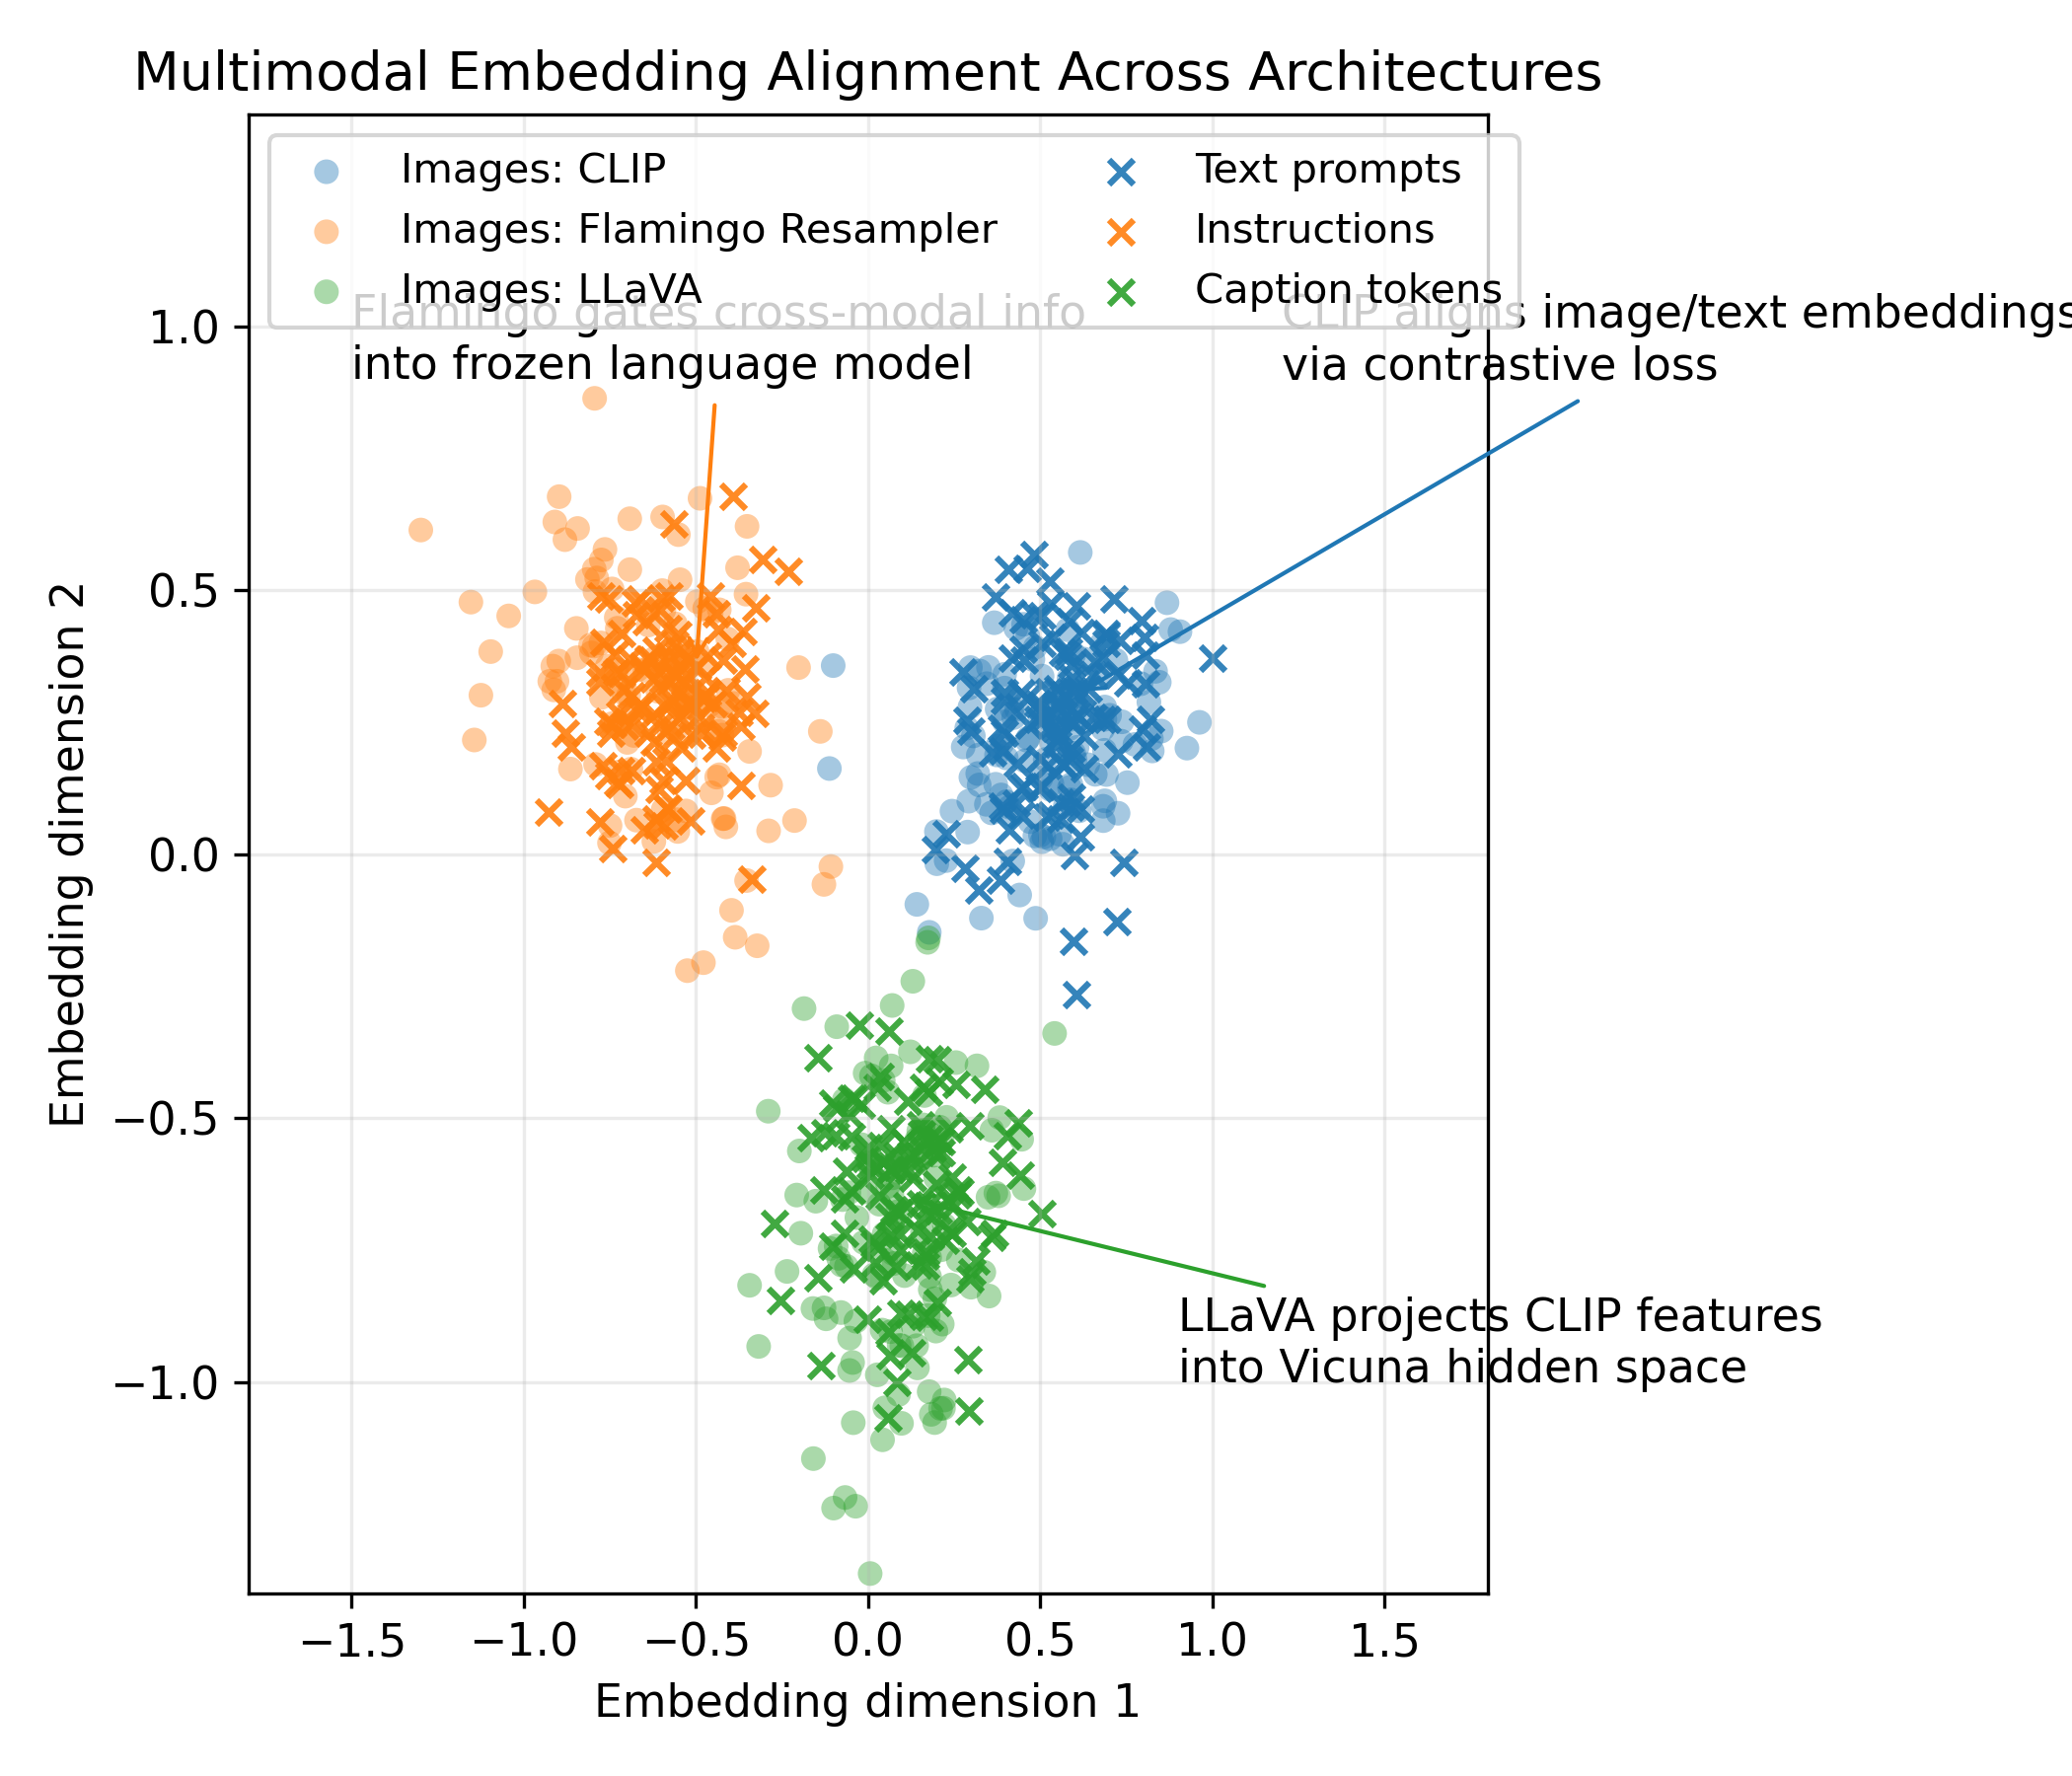
\includegraphics[width=0.85\textwidth]{clip_multimodal_alignment.png}
  \caption{Embedding geometry for CLIP, Flamingo, GPT-4, and LLaVA. CLIP learns aligned spaces; Flamingo and LLaVA bridge visual features into language models.}
  \label{fig:clip_multimodal_alignment}
\end{figure}
\FloatBarrier

\section{Training and Fine-tuning Large Models: LoRA, PEFT, RAG}
Scaling foundation models imposes prohibitive costs for full fine-tuning. Parameter-efficient fine-tuning (PEFT) techniques adapt pre-trained backbones with lightweight modules, while retrieval-augmented generation (RAG) grounds responses in external knowledge. Figures~\ref{fig:lora_rank_update} and~\ref{fig:rag_pipeline} illustrate key mechanisms.

\subsection{Low-Rank Adaptation (LoRA)}
LoRA freezes original weights $\mathbf{W}_0$ and learns low-rank updates $\Delta \mathbf{W} = \mathbf{B} \mathbf{A}$ with rank $r \ll d$:
\begin{equation}
  \mathbf{W} = \mathbf{W}_0 + \frac{\alpha}{r} \mathbf{B} \mathbf{A}, \quad \mathbf{A} \in \mathbb{R}^{r \times d_{\text{in}}}, \; \mathbf{B} \in \mathbb{R}^{d_{\text{out}} \times r}.
\end{equation}
During forward pass for hidden states $\mathbf{h}$:
\begin{equation}
  \mathbf{y} = \mathbf{W}_0 \mathbf{h} + \frac{\alpha}{r} \mathbf{B} (\mathbf{A} \mathbf{h}).
\end{equation}
Only $\mathbf{A}, \mathbf{B}$ are trained, reducing parameter count by $\mathcal{O}(r(d_{\text{in}} + d_{\text{out}}))$. Rank selection balances expressivity and storage; common values are $r \in \{4, 8, 16\}$.

\subsection{Prefix/Prompt Tuning and AdapterFusion}
PEFT encompasses multiple strategies:
\begin{itemize}
  \item \textbf{Prefix tuning:} Optimizes virtual tokens prepended to each layer's key/value matrices.
  \item \textbf{Prompt tuning:} Adjusts continuous prompt embeddings at the input layer only.
  \item \textbf{Adapters:} Inserts bottleneck MLPs with residual connections. AdapterFusion learns task-specific mixtures of previously trained adapters, enabling multi-task reuse.
\end{itemize}
Libraries such as Hugging Face PEFT unify these approaches, allowing composition (e.g., LoRA + prompt tuning).

\subsection{Retrieval-Augmented Generation (RAG)}
RAG mitigates hallucinations by retrieving documents $\{\mathbf{d}_k\}_{k=1}^{K}$ from index $\mathcal{D}$ conditioned on query $\mathbf{q}$:
\begin{equation}
  \mathbf{d}_k = \mathrm{Retrieve}(\mathbf{q}, \mathcal{D}), \qquad \mathbf{y} \sim p_{\theta}(\mathbf{y} \mid \mathbf{q}, \mathbf{d}_{1:K}).
\end{equation}
Dense retrievers (DPR, Contriever) encode queries/documents via bi-encoders trained with contrastive loss. Generation integrates retrieved passages via:
\begin{itemize}
  \item \textbf{Fusion-in-decoder (FiD):} Concatenate encoder outputs per passage before cross-attention.
  \item \textbf{RAG-token/RAG-sequence:} Marginalize over retrieved documents during autoregressive decoding.
\end{itemize}
Adaptive retrieval refreshes indexes periodically, while caching strategies reduce latency in production.

\subsection{Implementation Example}
\begin{lstlisting}[language=Python, caption={LoRA fine-tuning with retrieval-augmented prompting (Hugging Face PEFT).}]
from peft import LoraConfig, get_peft_model
from transformers import AutoModelForCausalLM, AutoTokenizer
from rag_pipeline import DenseRetriever, format_context

base_model = AutoModelForCausalLM.from_pretrained("meta-llama/Llama-2-7b-hf", device_map="auto")
tokenizer = AutoTokenizer.from_pretrained("meta-llama/Llama-2-7b-hf")

lora_config = LoraConfig(
    r=8,
    lora_alpha=32,
    lora_dropout=0.1,
    target_modules=["q_proj", "v_proj"],
)
model = get_peft_model(base_model, lora_config)

retriever = DenseRetriever(index_path="faiss.index")

def generate_with_rag(question: str):
    docs = retriever.search(question, top_k=5)
    prompt = format_context(question, docs)
    inputs = tokenizer(prompt, return_tensors="pt").to(model.device)
    outputs = model.generate(**inputs, max_new_tokens=256, temperature=0.7)
    return tokenizer.decode(outputs[0], skip_special_tokens=True)
\end{lstlisting}

\subsection{Production Considerations}
\begin{itemize}
  \item \textbf{Memory footprint:} LoRA weights stored separately ($\sim$ tens of MB) support rapid model switching.
  \item \textbf{Evaluation:} Align with human preference tests; offline Rouge/BLEU insufficient for conversational agents.
  \item \textbf{Safety:} Retrieval filters and response vetting prevent leakage of undesired content.
\end{itemize}

\begin{figure}[H]
  \centering
  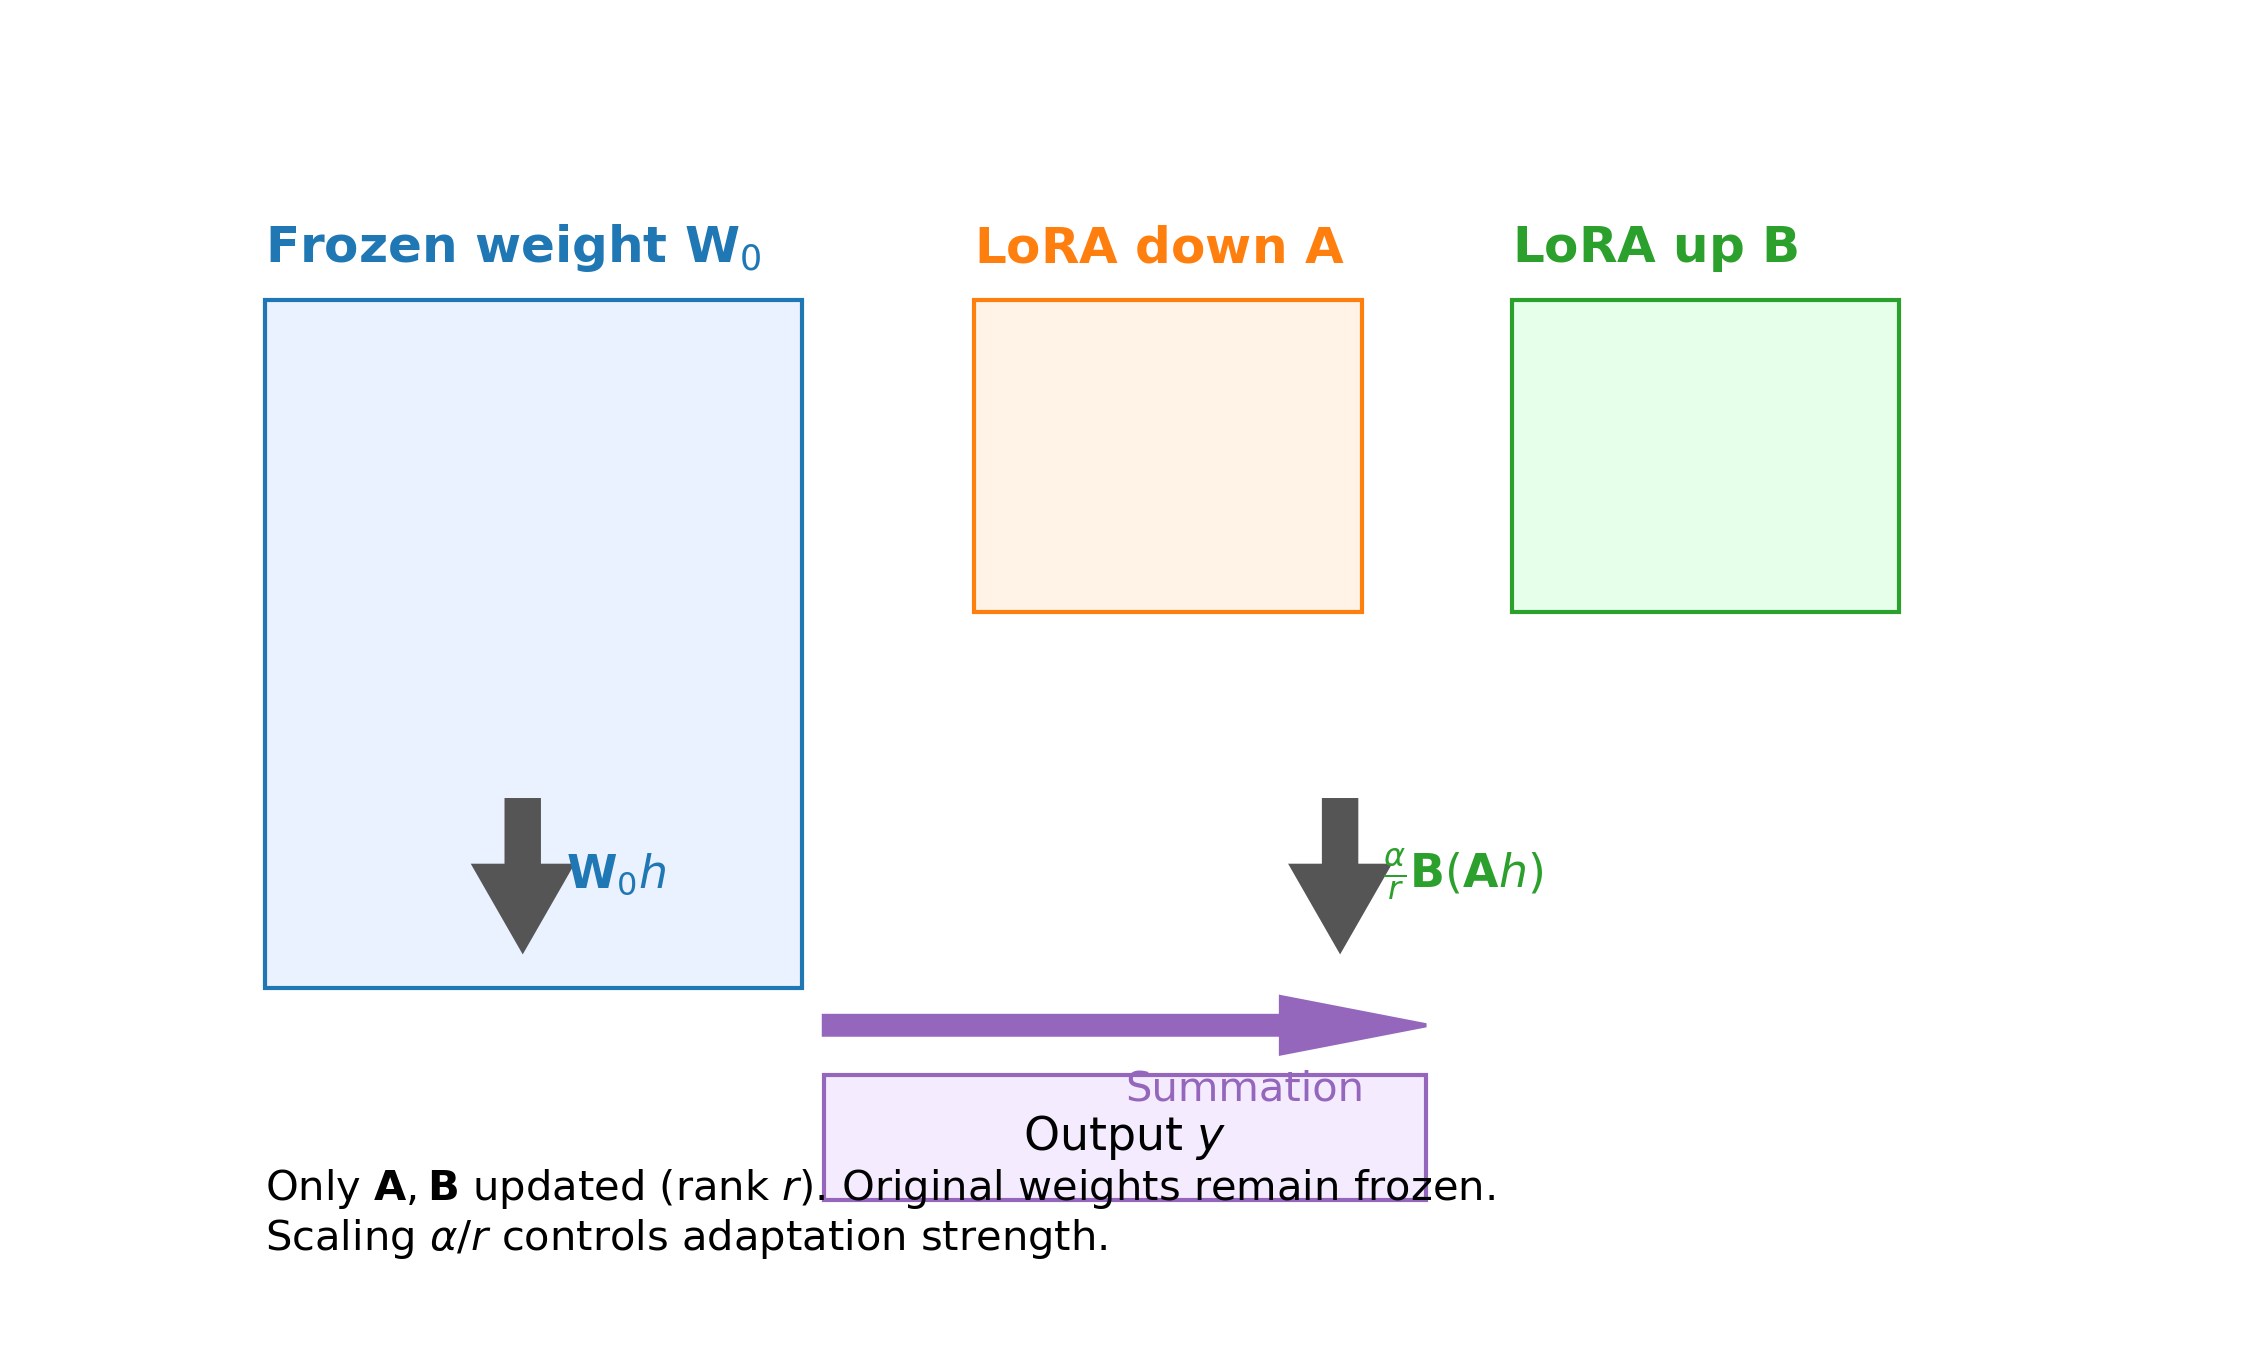
\includegraphics[width=0.85\textwidth]{lora_rank_update.png}
  \caption{LoRA inserts low-rank adapters into attention projections. Rank and scaling determine adaptation capacity.}
  \label{fig:lora_rank_update}
\end{figure}

\begin{figure}[H]
  \centering
  
\includegraphics[width=0.9\textwidth]{rag_pipeline.png}
  \caption{Retrieval-augmented generation pipeline with dense retriever, chunked index, and generator fusion strategies.}
  \label{fig:rag_pipeline}
\end{figure}
\FloatBarrier

\section*{Further Reading}
\begin{itemize}
  \item Alec Radford et al. ``Learning Transferable Visual Models From Natural Language Supervision.'' ICML 2021.
  \item Jean-Baptiste Alayrac et al. ``Flamingo: A Visual Language Model for Few-Shot Learning.'' NeurIPS 2022.
  \item Jonathan Ho et al. ``Scaling Instruction-Finetuned Language Models.'' 2022.
  \item Edward Raffel et al. ``Scaling Instruction-Finetuned Language Models.'' 2023.
  \item Tianyi Zhang et al. ``PEFT: Parameter-Efficient Fine-Tuning of Transformers.'' 2022.
\end{itemize}

\end{document}
